\section{Zielsetzung}
In diesem Versuch werden Amplituden und effektiver Dämpfungswiderstand eines gedämpften, sowie
die Frequenzabhängigkeit der Spannung und der Phasenverschiebung eines angeregten Schwingkreises
untersucht. Außerdem wird der Widerstand ermittelt, bei dem in einem gedämpften Schwingkreis der
aperiodische Grenzfall eintritt.

\section{Theorie}
Ein Schwingkreis besteht im einfachsten Fall aus einem Kondensator mit einer Kapazität $C$ und einer Spule mit der Induktivität $L$.
Die Energie in diesem System oszilliert zwischen dem elektrischen Feld des Kondensators und dem magnetischen Feld der Spule.
Falls ein idealer Draht vorliegt, bleibt diese \textbf{ungedämpfte Schwingung} für $ t \to \infty $ unverändert.

\subsection{Gedämpfte Schwingung}

Wenn  in dem Schwingkreis noch ein endlicher Widerstand $R$ eingebaut ist, dann wird dies als \textbf{gedämpft Schwingung}
bezeichnet, denn hier geht Energie in Form von Wärme über den Draht oder den Widerstand verloren. Dadurch fallen die Amplituden
der Schwingungen exponentiell ab.

\begin{figure}[h]
  \centering
  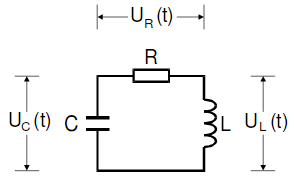
\includegraphics[scale=0.5]{gSchwingkreis.png}
  \caption{Schwingkreis einer gedämpften Schwingung.}
  \label{gSchwingung}
\end{figure}

Der Abfall der Amplituden lässt sich aus dem zweiten Kirchhoffschen Gesetz (Maschenregel) mit Hilfe der Spannungen aus der Abbildung \ref{gSchwingung}
herleiten:

\begin{equation*}
  U_R(t) + U_L(t) + U_C(t) = 0.
\end{equation*}

Mit den folgenden Definitionen der Spannung $U$, der Stromstärke $I$, der Induktivität der Spule $L$,
der Kapazität des Kondensators $C$, der Ladung $Q$ des Kondensators und des Widerstandes $R$

\begin{align*}
  U_R(t) &= R I(t) \\
  U_C(t) &= L \, \frac{\symup d I(t)}{\symup d t} \\
  U_L(t) &= \frac{Q(t)}{C} \, ,
\end{align*}

lässt sich eine lineare Differentialgleichung 2. Ordnung aufstellen

\begin{equation*}
  \ddot{I}(t) + \frac{R}{L} \dot{I}(t) + \frac{1}{LC} I(t) = 0 \, .
\end{equation*}

Die Lösung der Differentialgleichung lautet

\begin{equation}
  I'(t) = e^{-2 \pi \mu t} (A e^{i 2 \pi \nu t} + B e^{-i 2 \pi \nu t}) \, ,
  \label{Gleichung1}
\end{equation}

wobei $A$ und $B$ beliebige komplexe Zahlen sind und die Abkürzungen wie folgt definiert werden

\begin{align}
  2 \pi \mu &= \frac{R}{2L} \\
  2 \pi \nu &= \sqrt{\frac{1}{LC} - \frac{R^2}{4L^2}}
\end{align}

Für den weiteren Verlauf ist es notwendig zu ermitteln, ob $\nu$ reel oder imaginär ist. Deshalb wird eine
Fallunterscheidung durchgeführt:

\begin{itemize}
  \item $\nu $ ist reell, bzw. $\frac{1}{LC} > \frac{R^2}{4L^2}$

  Damit $I'(t)$ reell wird, muss $A=\overline{B}$ gelten, so erhält man durch den Ansatz

  \begin{align*}
    A &= \frac{1}{2} A_0 e^{i \eta}\\
    B &= \frac{1}{2} A_0 e^{-i \eta} \, ,
  \end{align*}
  wobei $A_0$ und $\eta$ reell sein sollen, die Funktion

  \begin{equation*}
    I(t) = A_0 e^{-2 \pi \mu t} cos(2 \pi \nu t + \eta).
  \end{equation*}

  Diese Gleichung stellt eine gedämpfte Schwingung mit der Freuquenz $\nu$ dar, dessen Amplitude exponentiell
  abfällt, mit der Schwingungsdauer

  \begin{equation*}
    T = \frac{1}{\nu} = \frac{2 \pi}{\sqrt{\frac{1}{LC} - \frac{R^2}{4L^2}}}
  \end{equation*}

  Die Abnahmegeschwindigkeit lässt sich aus dem Exponenten der e-Funktion herleiten. Daraus lässt sich
  die Abklingdauer $T_{\symup{ex}}$ definieren, als

  \begin{equation}
    T_{\symup{ex}} := \frac{1}{2 \pi \mu} = \frac{2L}{R} \, .
  \end{equation}

  \item $\nu $ ist imaginär, bzw. $\frac{1}{LC} < \frac{R^2}{4L^2}$

  Es gibt keinen oszillatorischee Anteil mehr in der Gleichung (\ref{Gleichung1}), da nurnoch die reelle
  Exponentialfunktion vorkommt. Es kommt zu einer aperiodischen Dämpfung. Abhängig von $A$ und $B$ strebt
  $I(t)$ monoton gegen 0 oder erreicht noch einen Extremwert. Für das Experiment von Bedeutung ist nur
  der Spezialfall

  \begin{equation}
    \frac{1}{LC} = \frac{R^2}{4L^2}
  \end{equation}

  hierbei geht die Funktion ohne Überschwingungen am schnellsten gegen 0.

\end{itemize}

\subsection{Erzwungene Schwingung}


Nun wird der RCL-Kreis durch eine äußere periodische Schwingung mit einer Eigenfrequenz ergänzt,
in diesem Fall mit einer sinusförmigen Wechselspannung $U(t)$, dies wird nun als \textbf{erzwungene Schwingung} bezeichnet.
Nach einer gewissen Einschwingzeit wird der RCL-Kreis mit derselben Frequenz wie die Wechselstromquelle schwingen.

\begin{figure}[h]
  \centering
  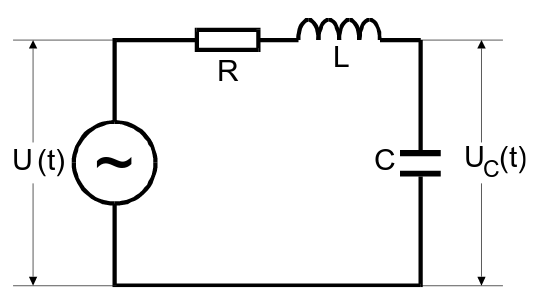
\includegraphics[scale=0.5]{eSchwingkreis.png}
  \caption{Schwingkreis einer erzwungenene Schwingung.}
  \label{eSchwingung}
\end{figure}
Mit

\begin{equation*}
  U(t) = U_0 e^{i \omega t}
\end{equation*}

wird die Differentailgleichung noch ergänzt. Die Differentialgleichung nimmt dann die Gestalt an:

\begin{equation*}
  \label{DGL2}
  L \dot{I}(t) + R I(t) + \frac{Q(t)}{C} = U_0 e^{i \omega t}
\end{equation*}
 bzw.
 \begin{equation*}
   \label{DGL3}
   LC \ddot{U}_C + RC \dot{U}_C + U_C = U_0 e^{i \omega t}
 \end{equation*}
 wobei $Q(t)$ die Ladung auf dem Kondensator entsprich.

 Um zu ermitteln, wie die Amplitude $U_{C_0}$ der Kondensatorspannung mit dem Phasenunterschied von der Erregerspannung
 mit der Amplitude $U_0$ und ihrer Frequenz abhängen, wird Ansatz

 \begin{equation*}
   U_C(\omega t) = U_{C_0} (\omega) e^{i \omega t}
 \end{equation*}

 genommen und setzt diesen in die DGL (\ref{DGL3}) ein, so erhält man für die Amplitude

 \begin{equation}
   \label{equation1}
   U_{C_0} = \frac{U_0 (1 - LC \omega^2 - i \omega RC)}{(1 - LC \omega^2)^2 + \omega^2 R^2 C^2 S}
 \end{equation}

 und die Phasenverschiebung $\phi (\omega)$ zwischen $U_C(t)$ und $U(t)$

 \begin{equation}
 \label{winkel}
   \phi(\omega) = \arctan \left(\frac{- \omega RC}{1 - LC \omega^2}\right)
 \end{equation}

Mit (\ref{equation1}) erhält man für die Kondensatorspannung in Abhängigkeit von $\omega$ die sogenannte Resonanzkurve
\begin{equation}
  \label{omega}
  U_C(\omega) = \frac{U_0}{\sqrt{(1-LC \omega^2)^2 + \omega^2 R^2 C^2}}
\end{equation}

Für die Frequenzen $\omega_1$ und $\omega_2$ bei denen die Phasenverschiebung genau $\frac{\pi}{2}$ bzw. $\frac{3 \pi}{4}$
beträgt, gilt dann

\begin{equation}
  \omega_{1,2} = \pm \frac{R}{2L} + \sqrt{\frac{R^2}{4L^2} + \frac{1}{LC}}
\end{equation}

Bei näherer Betrachtung der Gleichung \eqref{omega} ist zu erkennen, dass $U_C$ für $\omega \to \infty$ gegen 0 geht
und für $\omega \to 0$ gegen die Erregeramplitude $U_0$ strebt. $U_C$ erreich aber auch bei einer bestimmten Frequenz
ein Maximum, dieses Phänomen wird \textbf{Resonanz} bezeichnen. Die zugehörige Resonanzfrequenz lässt sich durch

\begin{equation}
  \omega_{res} = \sqrt{\frac{1}{LC} + \frac{R^2}{2L^2}}
\end{equation}

berechnen. Falls die Resonanzfrequenz ungefähr der Frequenz der Erregerspannung ($\omega_0 = \frac{1}{LC}$) entspricht, d.h.
$ \frac{1}{LC} >> \frac{R^2}{2L^2} $, so wird dies als Schwache Dämpfung bezeichnet. Für diesen Fall wird $U_C$ um
den Faktor

\begin{equation}
  q = \frac{1}{\omega_0 RC}
\end{equation}

 größer als $U_0$. $q$ wird auch als Güte bezeichnet. Die Breite der Resonanzkurve ist eine weitere wichtige Größe,
 sie wird aus der Differenz der beiden Frequenzen $\omega_-$ und $\omega_+$ gewonnen. Wobei $\omega_-$ und $\omega_+$
 die Eigenschaft besitzen, dass die zugehörigen Spannungen $U_C(\omega_-)$ und $U_C(\omega_+)$  um den Faktor
 $\frac{1}{\sqrt{2}}$ kleiner sind, als das Maximum $U_C(\omega_{res})$ bei der Resonanzfrequenz.
 Mit der Näherung

 \begin{equation*}
   \frac{R^2}{L^2} << \omega_0^2
 \end{equation*}

folgt für die Differenz der Frequenzen

\begin{equation}
\omega_+ - \omega_- \approx \frac{R}{L}
\end{equation}

 \section{Durchführung}

Der Versuchsaufbau ist in Abbildung \ref{AufbauBild} und in Abbildung \ref{AufbauSchaltung} dargestellt. Auf Abbildung \ref{AufbauBild} ist auf der rechten
Seite den Sinuswellengenerator erkenne, welcher mit dem Bauteil, in welchem der RCL-Schwingkreis eingebaut ist, verbunden
ist. Von dem RCL-Schwingkreis geht außerdem eine Verbindung zu dem 1. Eingang des Oszilloskop, um dort die erzeugte Schwingung
anzeigen zu können. Die zu erkennden Verbindung zwischen dem Sinuswellenenerator und dem Oszilloskop wird erst im späteren Verlauf
des Versuchs hinzugefügt.
\begin{figure}[h]
  \centering
  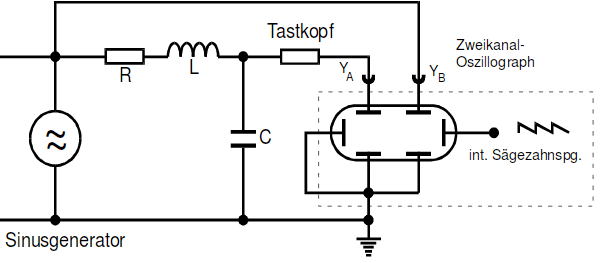
\includegraphics[scale=0.4]{aufbau2.png}
  \caption{Versuchsaufbau Schaltkreis.}
  \label{AufbauSchaltung}
\end{figure}
Im ersten Teil des Versuchs soll die Zeitabhängigkeit der Amplitude einer gedämpften Schwingung untersucht und
daraus den Dämpfungswiderstand ermittelt werden. Es wird für die Messung der kleinere von den beiden festen Widerständen
angeschlossen. Hierzu wird eine Rechteckspannung durch den Sinusgenerator erzeugt
und auf dem Oszilloskop sichtbar gemacht. Folgend werden alle Hoch- und Tiefpunkte in Abhängigkeit der Zeit vermessen
und notiert.
\begin{figure}[h]
  \centering
  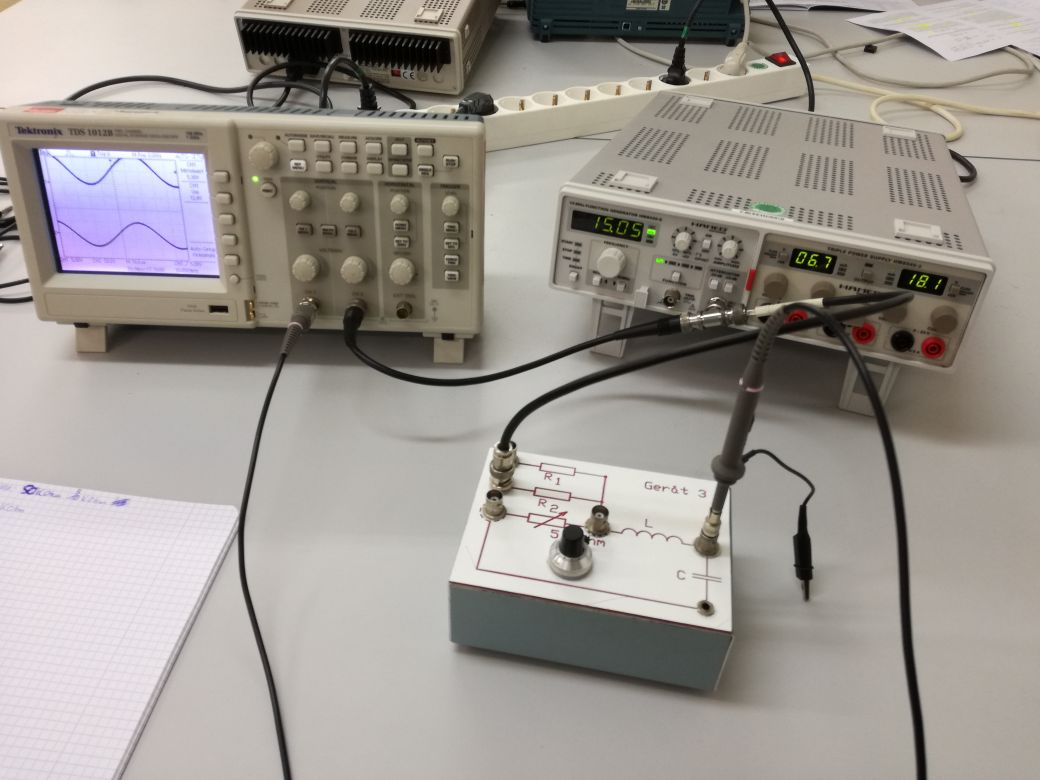
\includegraphics[scale=0.2]{V354Aufbau.jpeg}
  \caption{Versuchsaufbau.}
  \label{AufbauBild}
\end{figure}
Im zweiten Teil des Versuchs soll der aperiodische Grenzfall der Schwingung ermittelt werden. Hierzu wird die Schaltung
an den veränderbaren Widerstand angeschlossen, eine Rechteckspannung durch den Sinusgenerator erzeugt und auf dem
Oszilloskop sichtbar gemacht. Zunächst wird der veränderbare Widerstand auf den höchstmglichen Wert gestellt. Danach
wird der Widerstand verringert, bis eine erste Überschwingung zu erkennen ist. Daraufhin wird der Widerstand
etwas vergrößert, sodass gerade keine Überschwingung mehr vorhanden ist. Der Wert des Widerstandes wird notiert.

Der Aufbau der letzten beiden Versuchsteile ist identisch. Hierzu wird zusätzlich noch eine Verbindung von dem Sinuswellengenerator
zu dem Oszilloskop hergestellt, um eine unveränderte Sinusschwingung anzeigen zu lassen. Der Sinuswellengenerator erzeugt
bei beiden Teilen eine Sinusschwingung. Hierzu wird der größere von den beiden festen Widerständen angeschlossen.

Zunächst wird die Abhängigkeit der Kondensatorspannung von der Frequenz gemessen. Hierzu werden Frequenzen im Bereich
von 15kHz bis 60kHz in 5kHz-Schritten abgetastet und die jeweiligen Amplituden der Kondensatorspannungen abgemessen.
Da die Amplitude der Vergleichsspannung immer gleich bleibt, wird diese zuvor einmal gemessen und die Verbindung
kann im weiteren Verlauf vom Oszilloskop getrennt werden.
In dem Bereich der größten Amplituden werden weitere Messungen durchgeführt, diesmal in 1kHZ-Schritten, um den Peak
der Kondensatorspannung besser darstellen zu können.

Im letzten Teil des Versuches wird die Abhängigkeit der Phasenverschiebung von der Frequenz ermittelt.
Hierzu wird analog wie zuvor vorgegangen: Es werden Frequenzen im Beriech von 15kHz bis 60kHz abgetastet und die jeweilige
Schwingungsdauer $T$ und die Phasenverschiebung der Kondensatorspannnung gemessen. Hierbei kann die Ausgangsspannung nicht
vom Oszilloskop getrennt werden, da diese für die Messung der Phasenverschiebung notwendig ist. Wie im vorherigen Teil
des Versuchs, werden auch im kritischen Bereich der Resonanzfrequenz weitere Messwerte in 1kHz-Schritten aufgenommen.

\section{Auswertung}
Für alle gemittelten Werte wurde folgende Formel benutzt:
\begin{equation}
  \bar{x} = \frac{1}{n}\sum\limits_{i=1}^n x_{i}
\end{equation}

und deren Standardabweichung:
\begin{equation}
  \Delta\bar{x} = \sqrt{\frac{1}{n*(n-1)}\sum\limits_{i=1}^n (x_i - \bar{x})^2}
\end{equation}

Wurden berechnete Fehler für weitere Berechnungen benutzt, wurden diese mit der Gaußschen Fehlerfortpflanzung
berechnet:
\begin{equation}
  \Delta f = \sqrt{(\frac{\delta f(x)}{\delta x}\delta x)^2 + (\frac{\delta f(y)}{\delta y}\delta y)^2 + \cdots}
\end{equation}

Die Gerätedaten, die für die Berechungen benutzt wurden, lauten
\begin{align*}
  L & = \SI{3.53(3)e-3}{\milli\henry} \\
  C & = \SI{5.015(500)}{\milli\farad} \\
  R_1 & = \SI{30.3(1)}{\ohm} \\
  R_2 & = \SI{271.6(3)}{\ohm}
\end{align*}

\subsection{Zeitabhängigkeit der gedämpften Schwingung}
Tabelle 1 zeigt die mit Hilfe des Oszilloskops vermessenen Spannungsamplituden $U_\symup{C}$ mit den dazugehörigen
Zeiten $t$.

\begin{table}
  \centering
  \caption{Messwerte zur Bestimmung der Abklingdauer und des Dämpfungswiderstandes}
  \label{tab:1}
  \sisetup{table-format=2.3}
  \begin{tabular}{S S[table-format=3.0]}
    \toprule
    {$U_\symup{C}\:/\:\si{\volt}$} & {$t\:/\:\si{\micro\second}$} \\
    \midrule
    -7.52 & -6  \\
    -5.28 & 22  \\
    -3.76 & 48  \\
    -2.64 & 76  \\
    -1.68 & 102 \\
    -1.04 & 130 \\
    -0.56 & 156 \\
    -0.24 & 184 \\
    0     & 212 \\
    0.160 & 238 \\
    0.400 & 266 \\
    0.480 & 292 \\
    0.500 & 319 \\
    0.540 & 346 \\
    0.560 & 373 \\
    0.560 & 400 \\
    0.620 & 427 \\
    0.640 & 455 \\
    0.700 & 415 \\
    0.700 & 440 \\
    0.720 & 388 \\
    0.760 & 360 \\
    0.800 & 333 \\
    0.880 & 307 \\
    0.920 & 279 \\
    1.06  & 252 \\
    1.22  & 225 \\
    1.42  & 198 \\
    1.68  & 171 \\
    2.0   & 144 \\
    2.64  & 117 \\
    3.28  & 91  \\
    4.24  & 63  \\
    5.68  & 36  \\
    7.6   & 9 \\
    \bottomrule
  \end{tabular}
\end{table}

Abbildung 2 zeigt den Abklingvorgang des gedämpften $RCL$-Kreises mit eingezeichneter
Einhüllenden. Diese Einhüllende hat die Form
\begin{equation}
  A = A_0e^{-2\symup{\pi}\mu\symup{t}}
\end{equation}

\begin{figure}[h]
  \centering
  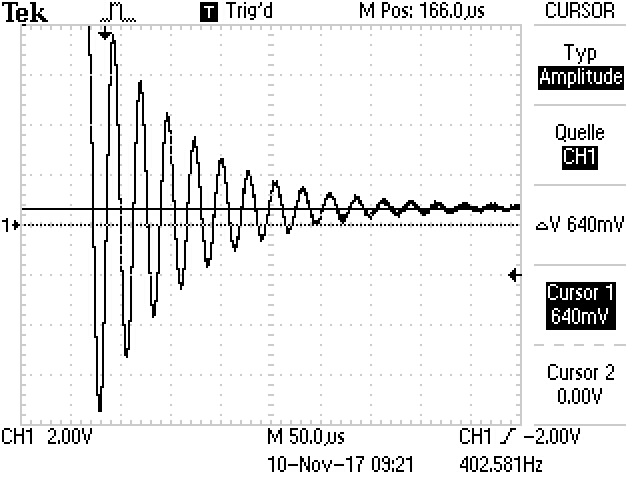
\includegraphics[scale=0.8]{Schwingung.JPG}
  \caption{Bild vom Oszilloskop, gedämpfte Schwingung}
  \label{Bild}
\end{figure}

\begin{figure}
   \centering
   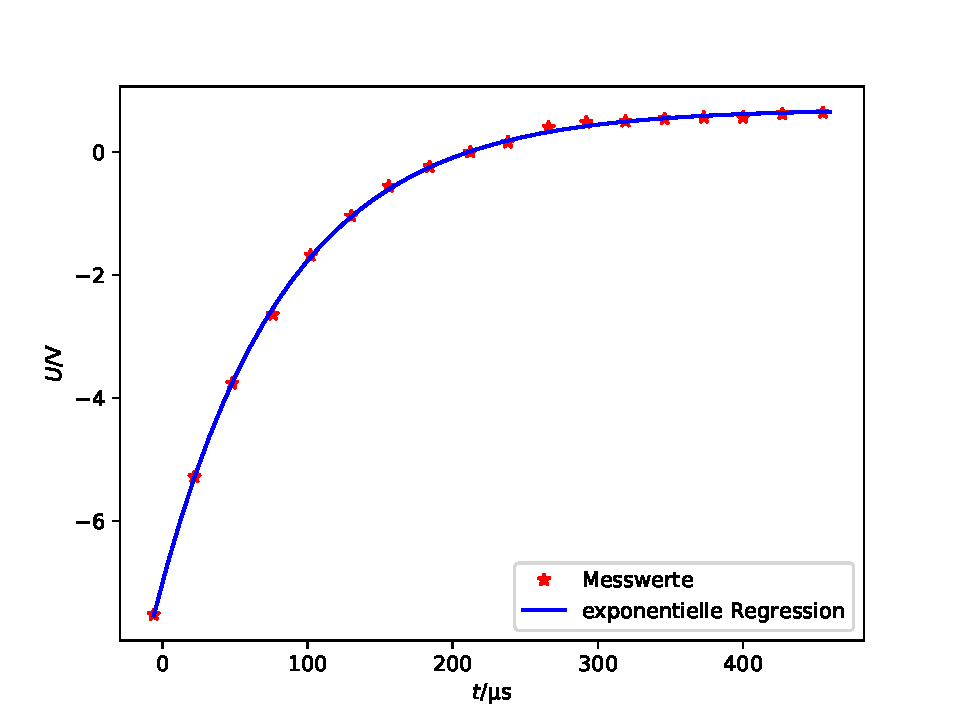
\includegraphics[scale = 0.5]{plotA1.pdf}
   \caption{Messwerte und exponentieller Fit des  unteren Teils der Einhüllenden}
   \label{Abb:2}
 \end{figure}

Die Werte zur Erstellung des exponentiellen Fits wurden aus Tabelle 1 entnommen und mittels dem Programm
"scipy optimize" ergeben sich folgende Werte für $\mu$ und $U_\symup{0}$:

\begin{equation}
  U_\symup{0} = \SI{0.6991(16)}{\volt}
%    U_\symup{0} = (0.6991 ± 0.016) \symup{V}
\end{equation}
\begin{equation}
  \symup{\mu} = \SI{1812(19)}{\per\second}
\end{equation}

Aus Gleichung (5) und (8) folgt ein effektiver Dämpungswiderstand $R_\symup{eff}$ und eine Abklingzeit $T_\symup{ex}$ von:

\begin{align*}
  R_\symup{eff} &= \SI{80.4(11)}{\ohm} \\
  T_\symup{ex} &= \SI{87.8(9)}{\micro\second}
\end{align*}

%\begin{equation}
%  T_\symup{ex} = (87.8 ± 0.9) \symup{\mu}\si{\second}
%\end{equation}

Es zeigt sich eine Abweichung von $R_1$ um $\SI{30.1}{ohm}$

\subsection{Dämpungswiderstand des aperiodischen Grenzfalls}

Mit Hilfe der Gleichung
\begin{equation*}
  R_\symup{ap} = \sqrt{\frac{4L}{C}}
\end{equation*} und Gleichung 9
wird folgender Wert für den Dämpfungswiderstand, bei dem der
aperiodische Grenzfall eintritt, berechnet:
\begin{equation*}
  R_\symup{ap} = \SI{1.68(8)}{\kilo\ohm}
\end{equation*}
Gemessen wurde ein Wert von \SI{1.395}{\ohm}, was eine Abweichung von \SI{0.285}{\kilo\ohm} im Mittel bedeutet.


\subsection{Frequenzabhängigkeit der Kondensatorspannung}

\begin{table}
  \centering
  \caption{Messwerte zur Untersuchung der Ferquenzabhängigkeit der Kondensatorspannung}
  \label{tab:2}
  \begin{tabular}{c c c}
    \toprule
    {$\nu / 10^3$ Hz} & {$U_\symup{C}$ / V} & {$U_\symup{C} / U_0$} \\
    \midrule
    15  &  5.98  &  1.187 \\
    20  &  6.86  &  1.361 \\
    25  &  8.34  &  1.655 \\
    30  &  10.9  &  2.163 \\
    31  &  11.5  &  2.282 \\
    32  &  12.1  &  2.401 \\
    33  &  12.6  &  2.500 \\
    34  &  13.0  &  2.579 \\
    35  &  13.2  &  2.619 \\
    36  &  13.3  &  2.639 \\
    37  &  13.0  &  2.579 \\
    38  &  12.5  &  2.480 \\
    39  &  11.9  &  2.361 \\
    40  &  11.2  &  2.222 \\
    45  &  7.45  &  1.478 \\
    50  &  5.14  &  1.020 \\
    55  &  3.76  &  0.746 \\
    60  &  2.9   &  0.575 \\
    \bottomrule
  \end{tabular}
\end{table}

 \begin{figure}
  \centering
  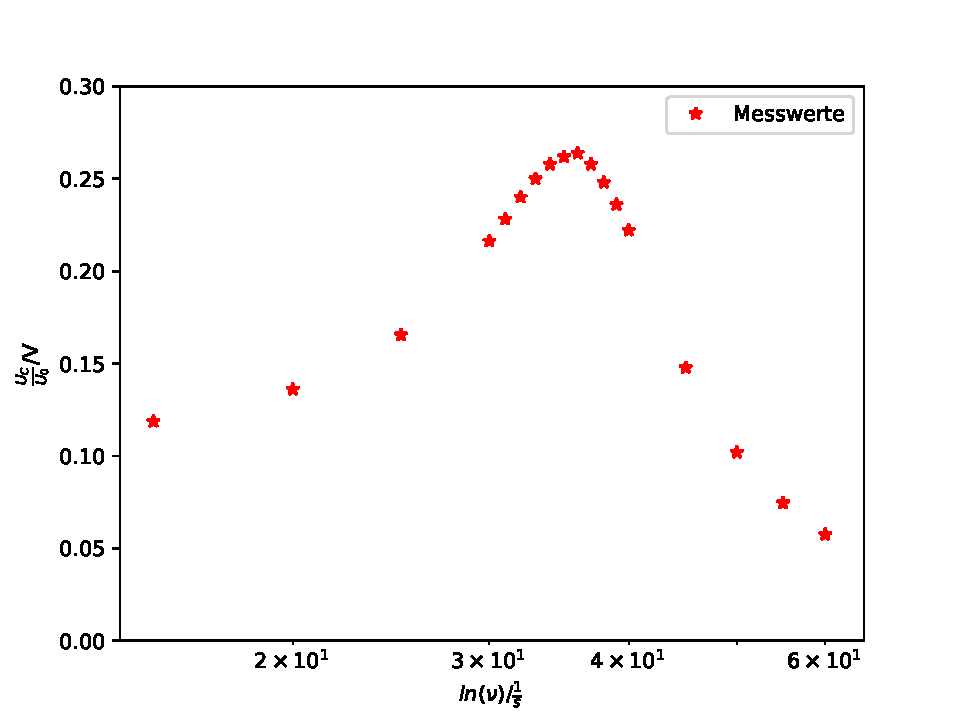
\includegraphics[scale = 0.7]{plotC1.pdf}
  \caption{Hier wird der Quotient aus Erreger- und Kondensatorspannung gegen $\nu$ halblogarithmisch aufgetragen.}
  \label{Abb:3}
\end{figure}

 \begin{figure}
  \centering
  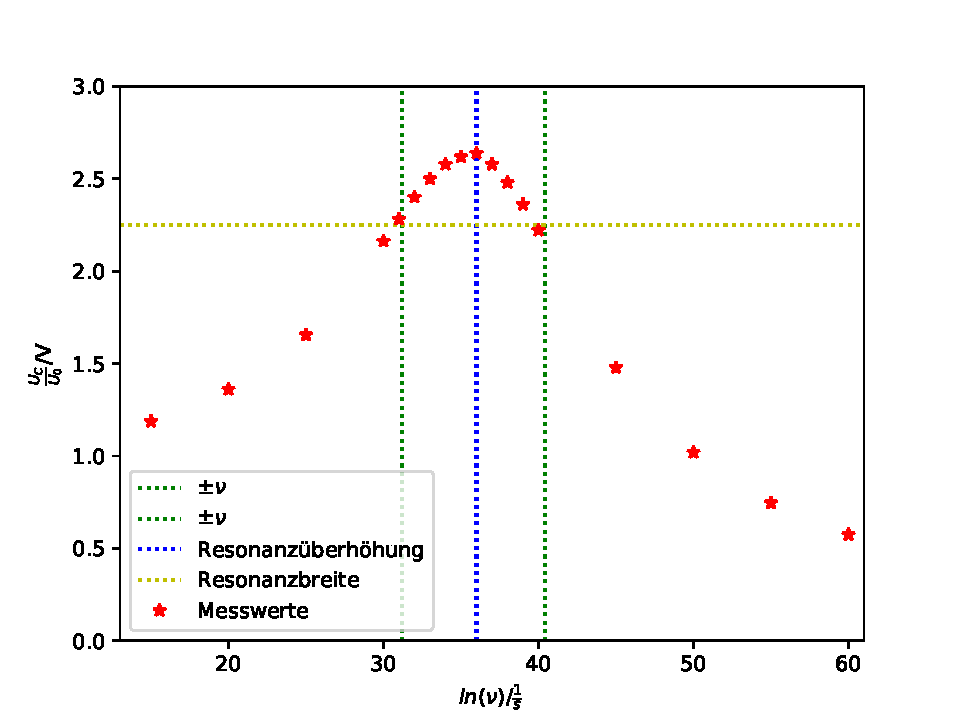
\includegraphics[scale = 0.7]{plotC2.pdf}
  \caption{Hier wird der Quotient aus Erreger- und Kondensatorspannung gegen $\nu$ linear aufgetragen. Außerdem zeigt
  die Abbildung lediglich den Ausschnitt um die Resonanzüberhöhung}
  \label{Abb:4}
 \end{figure}

In der Tabelle 2 sind die Werte für die anregende Frequenz $\nu$, die Kondensatorspannung $U_\symup{C}$ und die berechneten
Quotienten aus der Kondensatorspannung und der Erregerspannung eingetragen. Dieser Quotient wird in Abbildung 9 gegen die
Erregerfrequenz sowohl auf einer halblogarithmischen als auf einer linearen Skala (Abbildung 10) aufgetragen.
Beide Graphen zeigen das zu erwartende Bild, einer zunächst ansteigenden Kurve, die nach dem Erreichen ihres Maximums, der
Resonanzfrequenz, wieder abfällt. Mit Hilfe der Gleichung 5 und 6 wird der theoretische Wert für die Resonanzüberhöhung
$q$, sowie die Resonanzbreite $\nu_+$ - $\nu_-$ berechnet. Aus dem Diagramm können die experimentell ermittelten Werte für beides
gut abgelesen werden.
Sie betragen für die Resonanzbreite $\nu_1 - \nu_2 = 9.2\si{\kilo\Hz}$ und für die Resonanzüberhöhung $q= 2.7$
Die Theoriewerte betragen

\begin{align*}
  q &= 2.15 \pm 0.21 \\
  \nu_+ - \nu_- &= \SI{8.59(8)}{\kilo\Hz}
\end{align*}


\subsection{Frequenzabhängigkeit der Phase zwischen Erreger- und Kondensatorspannung}
Um die Frequnezabhängigkeit darzustellen, wird die Phasenverschiebung $\phi$ gegen die Frequenz der Erregerspannung $\nu$
wieder in einer halb logarithmischen Skalierung gegeneinander aufgetragen.Die Werte für $\phi$ und $\nu$ können Tabelle 3
entnommen werden.
$\phi$ wird mit Hilfe folgender Formel bestimmt:
\begin{equation*}
  \phi = \frac{\Delta t}{T}
\end{equation*}

\begin{table}
  \centering
  \caption{Messwerte für die Frequnez und die Phasenverschiebung zwischen Erreger und Kondensatorspannung}
  \label{tab:3}
  \begin{tabular}{c c c c}
    \toprule
    $\nu$ / \si{\kilo\hertz} & $\Delta t$ / \si{\per\micro\second} & $T = \frac{1}{\nu}$ \si{\micro\second} & $\phi$ / $\degree$ \\
  %  $\nu$ / kHz & $\Delta * t / $10^{-})$s & {$T = \sfrac{1}{\nu} / 10^{-6}$s & {$\phi / \degree$} \\
    \midrule
    15  &  1.2  &  66.5  &  6 \\
    20  &  1.6  &  50.2  &  11 \\
    25  &  2.2  &  40.2  &  19 \\
    30  &  3.7  &  33.4  &  40 \\
    31  &  3.9  &  32.2  &  47 \\
    32  &  4.4  &  31.2  &  51 \\
    33  &  4.8  &  30.4  &  57 \\
    34  &  5.4  &  29.4  &  66 \\
    35  &  5.8  &  28.6  &  73 \\
    36  &  6.1  &  27.8  &  79 \\
    37  &  6.6  &  27.0  &  88 \\
    38  &  7.1  &  26.4  &  97 \\
    39  &  7.7  &  25.6  &  108 \\
    40  &  7.9  &  25.0  &  114 \\
    45  &  8.5  &  22.3  &  137 \\
    50  &  8.4  &  20    &  151 \\
    55  &  7.8  &  18.3  &  153 \\
    60  &  9.3  &  16.7  &  200 \\
    \bottomrule
  \end{tabular}
\end{table}

 \begin{figure}
  \centering
  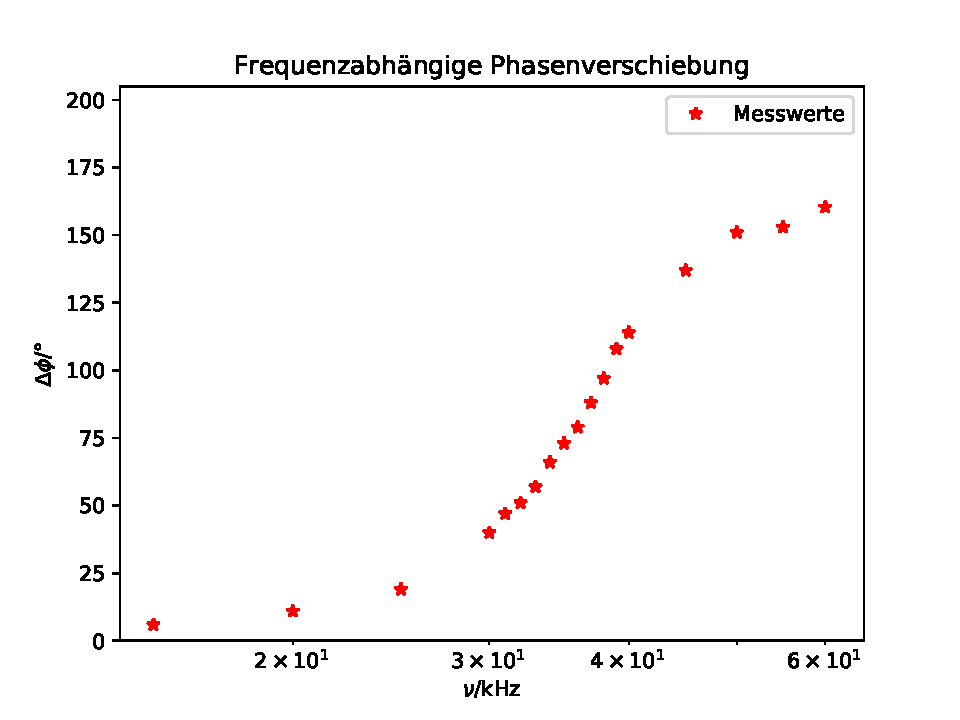
\includegraphics[scale = 0.7]{plotD1.pdf}
  \caption{Hier wird die Frequenz $\nu$ halblogarithmisch gegen die Phasenverschiebung$\nu$ aufgetragen.}
  \label{Abb:5}
 \end{figure}

\begin{figure}
  \centering
  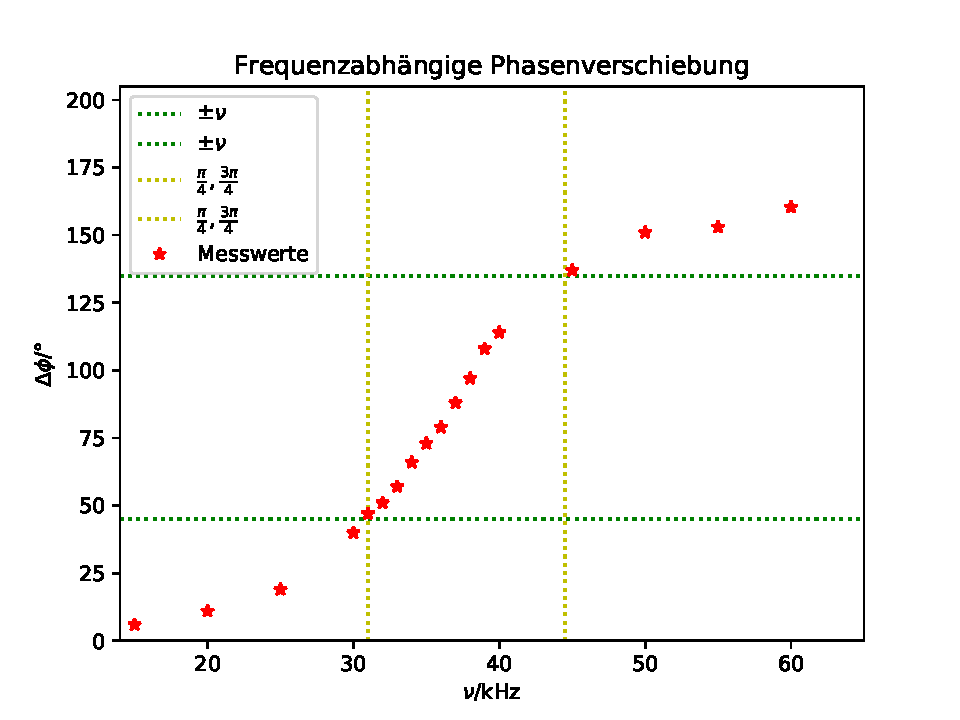
\includegraphics[scale = 0.7]{plotD2.pdf}
  \caption{Hier wird die Frequenz $\nu$ gegen die Phasenverschiebung $\nu$ aufgetragen.}
  \label{Abb:6}
 \end{figure}


 Abbildung  5 zeigt die halblogarithmische Darstellung, Abbildung 6 zeigt einen Ausschnitt des Frequenzbereichs um
 $\phi = 90 \degree$ in einer linearen Skalierung, um das Ablesen der Frequenzen zu erleichtern. Hieraus wird die
 Resonanzfrequenz $\nu_\symup{res}$ und $\nu_1$ und $\nu_2$, bei denen die Phasenverschiebung genau $\frac{\pi}{4}$,
 beziehungweise $\frac{3*np.pi}{4}$ beträgt, abgelesen.
 Die experimentell ermittelten Werte betragen:
 \begin{align*}
   \nu_1           &= 31 \\
   \nu_2           &= 44.5 \\
   \nu_\symup{res} &= 36
 \end{align*}

 Die Theoriewerte werden mit Hilfe der Gleichungen 8 und 9 berechnet und ergeben folgende Werte:

 Die Fehlerrechnung hierfür, wurde wie in allen Berechnungen, die fehlerbehaftete Größen enthalten mit Hilfe der Gaußschen
 Fehlerfortpflanzung berechnet.

\section{Diskussion}
Bei der Bestimmung des effektiven Dämpfungswiderstandes zeigt sich eine große Abweichung des Theoriewertes von tatsächlich gemessenen Wert
von $\SI{30.1}{\ohm}$, welche, genauso wie die relativ große Abweichung des Theoriewertes vom experimentell ermittelten Wert des Widerstandes
beim aperiodischen Grenzfall durch nicht beachtete Widerstände zu erklären ist. Hier ist besonders der Innenwiderstand des Generators zu bedenken.
Im Falle des Widerstandes, bei dem der aperiodische Grenzfall eintritt, muss die begrenzt maximale Auflösung des Oszilloskops und die Ungenauigkeit des rgelbaren
Widerstandes erwähnt werden, die ein exaktes Ablesen der gemessenen Werte erschwerten.\\
Die Abweichung bei der Bestimmung der Resonanzüberhöhung, also der Güte des Schwingkreises zeigt nicht allzu große Unterschiede zwischen dem experimentell ermittelten
Wert von 2.7 und dem theoretischen von $2.15 \pm 0.21$. Die etwas größere Abweichung der Theoriewerte der Resonanzbreite vom experimentell Ermittelten, lassen sich durch
die Methode zur Bestimmung der Werte erklären. Bei der graphischen Auswertung entstehen durch Abschätzungen zwangsläufig Fehler. Die Aufzeichnung weiterer Messwerte
könnte diese Fehler minimieren. Gleiches gilt für die experimentelle Ermittlung von $\nu_1$ und $\nu_2$. Auch hier könnten weitere Messwerte das graphisch ermittelte
Ergebnis von Fehlern befreien.
Abschließend ist zu sagen, dass der Versuch Ergebnisse mit unterschiedlich großen Abweichungen liefert. Teilweise sind die experimentell ermittelten Werte nah
an den Theoriewerten und auch die entstandenen Plots zeigen allesamt die erwarteten Verläufe, was auf einen sorgfältigen Messvorgang hindeuten kann.
Die Grenzen der Genauigkeit sind durch die vorgegebenen Apparaturen gegeben. So konnte man beispielsweise die Erregerspannung nie ganz exakt auf den gewünschten Wert
einstellen und auch der bereits erwähnte regelbare Widerstand war nur sehr ungenau zu bedienen.


\newpage
\nocite{*}
\printbibliography
